\section{Concepts} \label{sec:concepts}

\newpage

\subsection{Applying Constraints} \label{sec:applying_constraints}

    \subsubsection{Requires Clauses} \label{sec:requires_clauses}

        \lstinputlisting[linerange={6-13}]{examples/misc.cc}

        \begin{lstlisting}
[]<typename T>(T x, T y) requires EqualityComparable<T> {
    return x == y;
}; \end{lstlisting}

        \lstinputlisting[linerange={18-22,52-61,138-138}]{examples/matrix.hh}

        \lstinputlisting[linerange={24-28}]{examples/misc.cc}

        \lstinputlisting[linerange={42-52}]{examples/misc.cc}

        \newpage

    \subsubsection{Overload Resolution} \label{sec:overload_resolution}

        \begin{figure}[h]
            \centering
            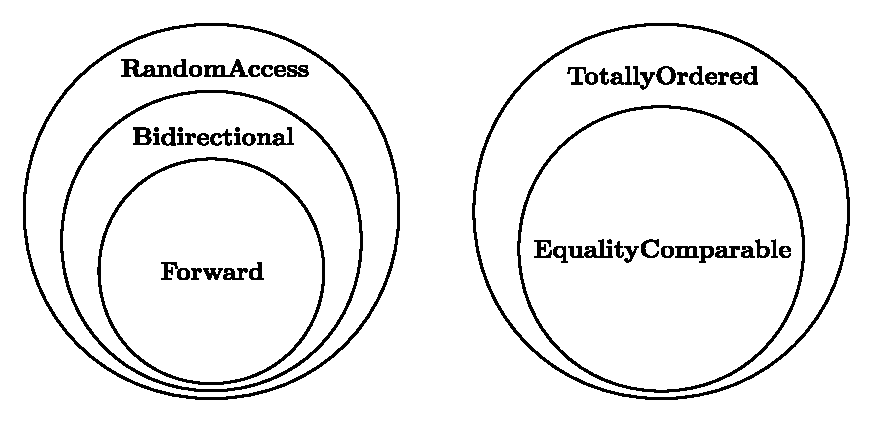
\includegraphics[width=0.7\textwidth]{figures/overloading.eps}
        \end{figure}

        \lstinputlisting[linerange={47-50,52-59,61-62}]{examples/advance.cc}

        \newpage

    \subsubsection{Logical Operations} \label{sec:logical_operations}

        \begin{figure}[h]
            \centering
            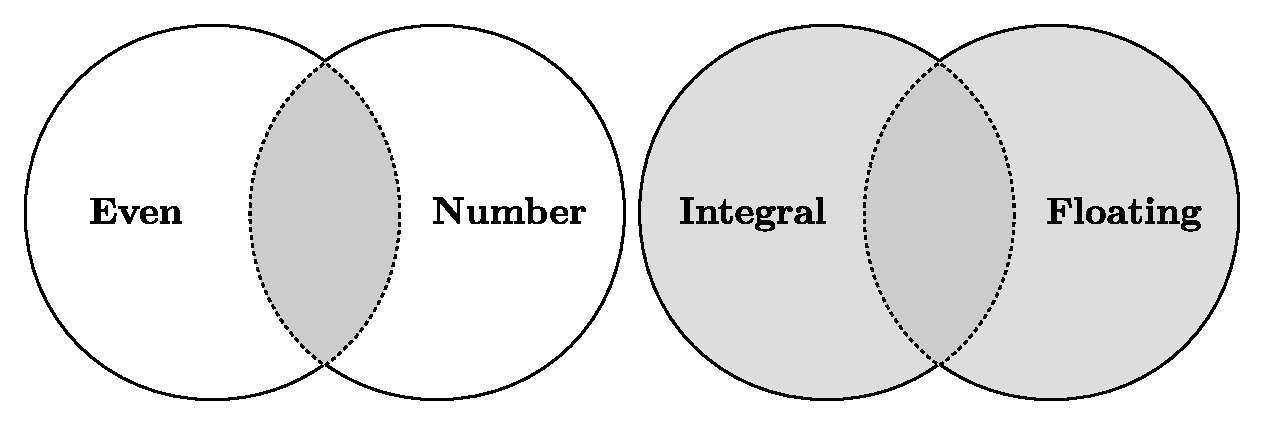
\includegraphics[width=0.7\textwidth]{figures/logical_operations.eps}
        \end{figure}

        \subsubsection*{Conjunctions} \label{sec:conjunctions}

        \lstinputlisting[linerange={30-35}]{examples/misc.cc}

        \subsubsection*{Disjunctions} \label{sec:disjunctions}

        \lstinputlisting[linerange={15-22}]{examples/misc.cc}

        \newpage

\subsection{Defining Requirements} \label{sec:defining_requirements}

    \subsubsection{Requires Expressions} \label{sec:requires_expressions}

        \lstinputlisting[linerange={152-169}]{examples/concepts.h}

        \subsubsection*{Simple Requirements} \label{sec:simple_requirements}

        \begin{lstlisting}
template<typename T>
concept ForwardIterator = requires {
    T();
    T{};
}; \end{lstlisting}

        \subsubsection*{Type Requirements} \label{sec:type_requirements}

        \begin{lstlisting}
template<typename T>
concept ForwardIterator = requires {
    typename std::iterator_traits<T>::value_type;
    typename std::iterator_traits<T>::difference_type;
    typename std::iterator_traits<T>::reference;
    typename std::iterator_traits<T>::pointer;
    typename std::iterator_traits<T>::iterator_category;
}; \end{lstlisting}

        \subsubsection*{Compound Requirements} \label{sec:compound_requirements}

        \begin{lstlisting}
template<typename T>
concept ForwardIterator = requires(T x) {
    {  *x } -> typename std::iterator_traits<T>::reference;
    { ++x } -> T&;
    { x++ } -> T;
} && requires(T x, T y) {
    { std::swap(x, y) } noexcept;
    { std::swap(y, x) } noexcept;
}; \end{lstlisting}

        \subsubsection*{Nested Requirements} \label{sec:nested_requirements}

        \lstinputlisting[linerange={191-199}]{examples/concepts.h}

        \newpage

\subsection{Giving Names to Concepts} \label{sec:giving_names_to_concepts}

    \lstinputlisting[linerange={175-180}]{examples/concepts.h}

    \lstinputlisting[linerange={182-184,186-186,188-189}]{examples/concepts.h}

    \subsubsection{``Good'' Concepts} \label{sec:good_concepts}
